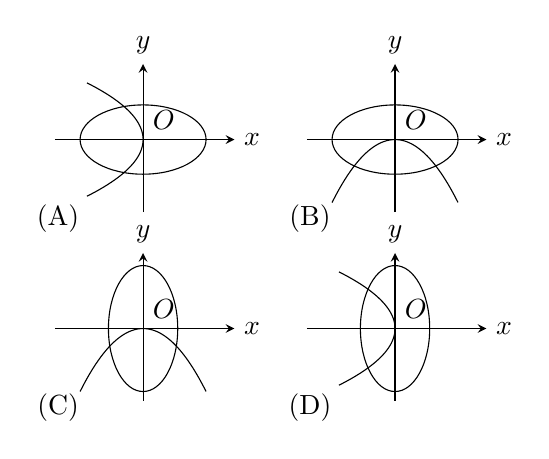
\begin{tikzpicture}[scale=.8,>=stealth]
\foreach \x/\y/\kind/\lab in {0/0/a/A,4/0/b/B,0/-3/c/C,4/-3/d/D}{
\begin{scope}[shift={(\x,\y)}]
\draw[->] (-1.4,0)--(1.45,0) node[right] {$x$}; \draw[->] (0,-1.15)--(0,1.2) node[above] {$y$};
\if\kind a \draw (0,0) ellipse (1 and .55); \draw[domain=-.9:.9,samples=50] plot ({-1.1*\x*\x},{\x});\fi
\if\kind b \draw (0,0) ellipse (1 and .55); \draw[domain=-1:1,samples=50] plot ({\x},{-\x*\x});\fi
\if\kind c \draw (0,0) ellipse (.55 and 1); \draw[domain=-1:1,samples=50] plot ({\x},{-\x*\x});\fi
\if\kind d \draw (0,0) ellipse (.55 and 1); \draw[domain=-.9:.9,samples=50] plot ({-1.1*\x*\x},{\x});\fi
\node[above right] at (0,0) {$O$}; \node at (-1.35,-1.25) {(\lab)};
\end{scope}}
\end{tikzpicture}
